\section{Integration Strategy}

\subsection{Entry Criteria}
\todo{da rivedere, guarda keep}
The following conditions have to be verified before entering the integration testing phase in order for it to produce meaningful results.\\
All of the components of the PowerEnJoy system must have passed unit testing with high percentage of covering, so that it is much likely that any problem discovered by integration testing is actually due to integration problems.

\subsection{Elements to be integrated}
Identify the components to be integrated, refer to your design document to identify such components in a way that is consistent with your design.

\subsection{Integration Testing Strategy}
A Bottom-up approach was chosen because most of the functionalities and the complexity is located in lower level components of our system, hence it is a better choice to test them first and ensure that they work well together before higher level components.

\subsection{Sequence of Component/Function Integration}
Depends on strategy chosen, this is a proposed structure.

\subsubsection{Software Integration Sequence}
For each subsystem, identify the sequence in which the software components will be integrated within the subsystem; relate this sequence to any product features that are being built up.

\paragraph{RentManager} 
The diagram above shows the needed precedences in the integration phase inside the \emph{RentManager} component.
\paragraph{}

		\begin{figure}[h]
			\centering
			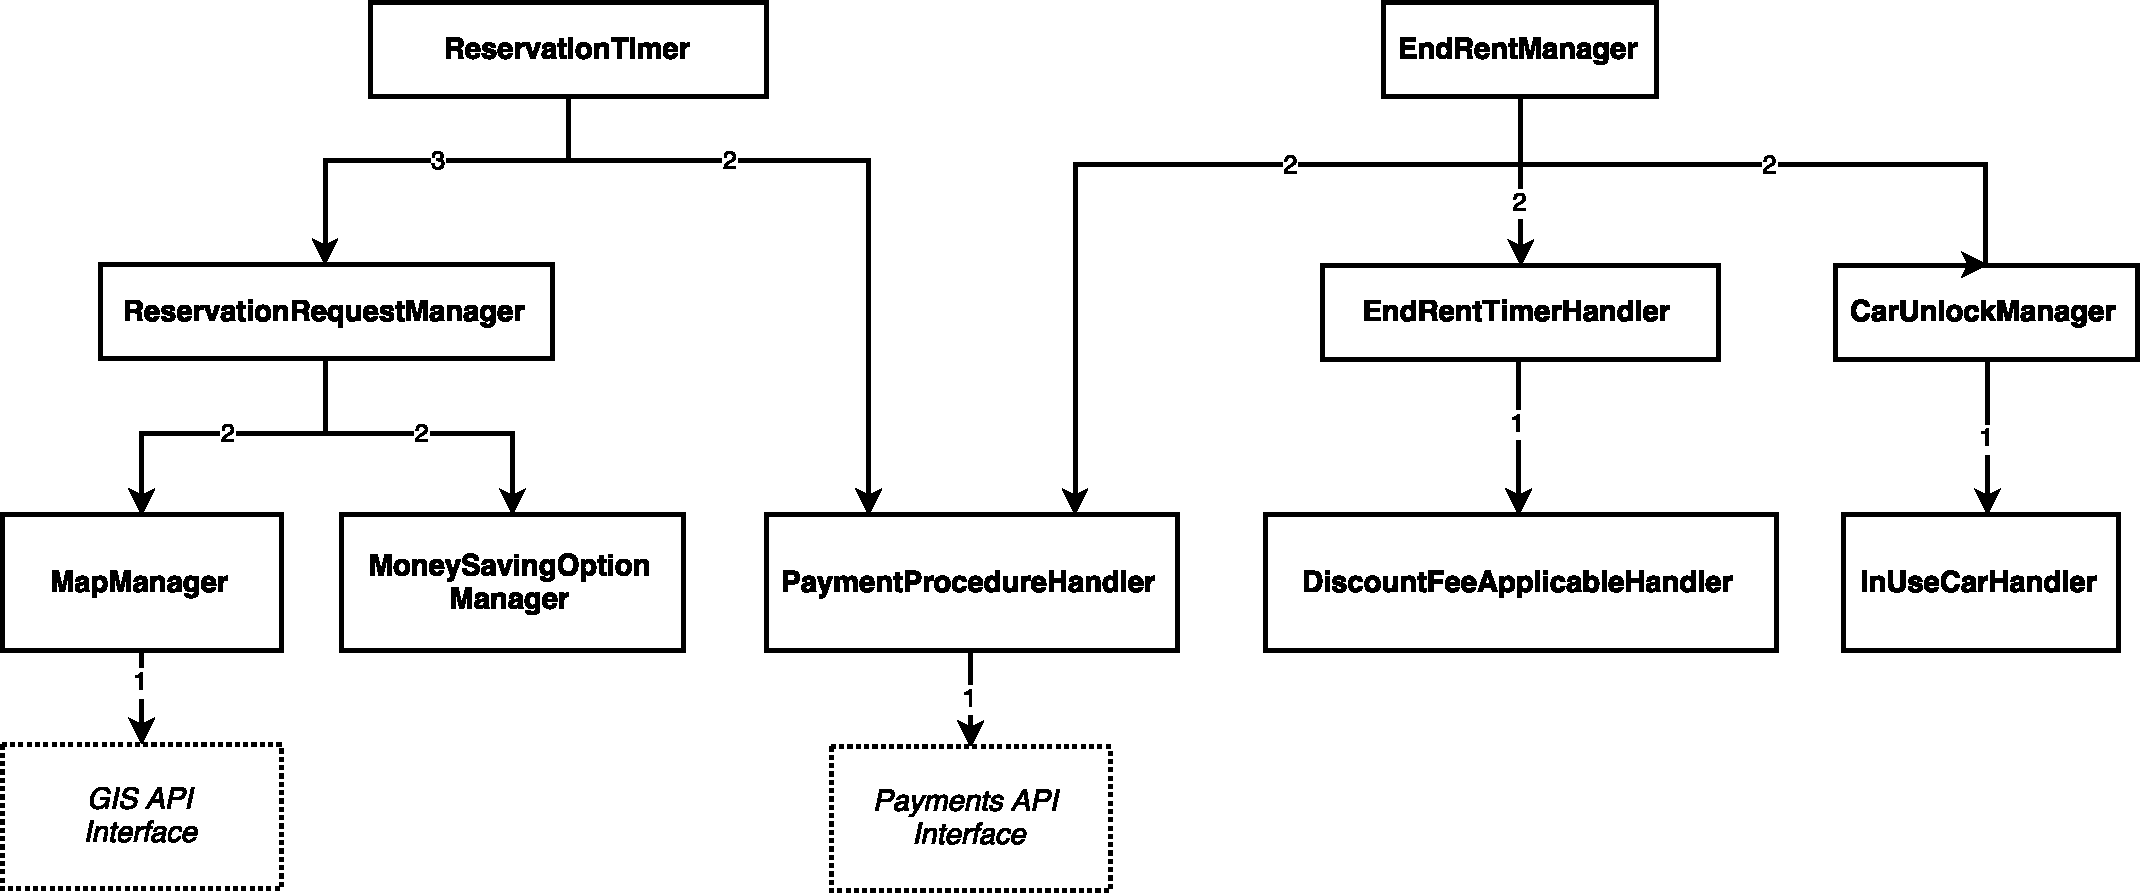
\includegraphics[width=\linewidth]{img/rentManagerIntegration}
			\caption{
				\label{fig:rentManagerIntegration} 
				\emph{RentManager integration}
			}
		\end{figure}
		
\paragraph{MaintenanceManager} 
The diagram above shows the needed precedences in the integration phase inside the \emph{MaintenanceManager} component.
\paragraph{}

		\begin{figure}[h]
			\centering
			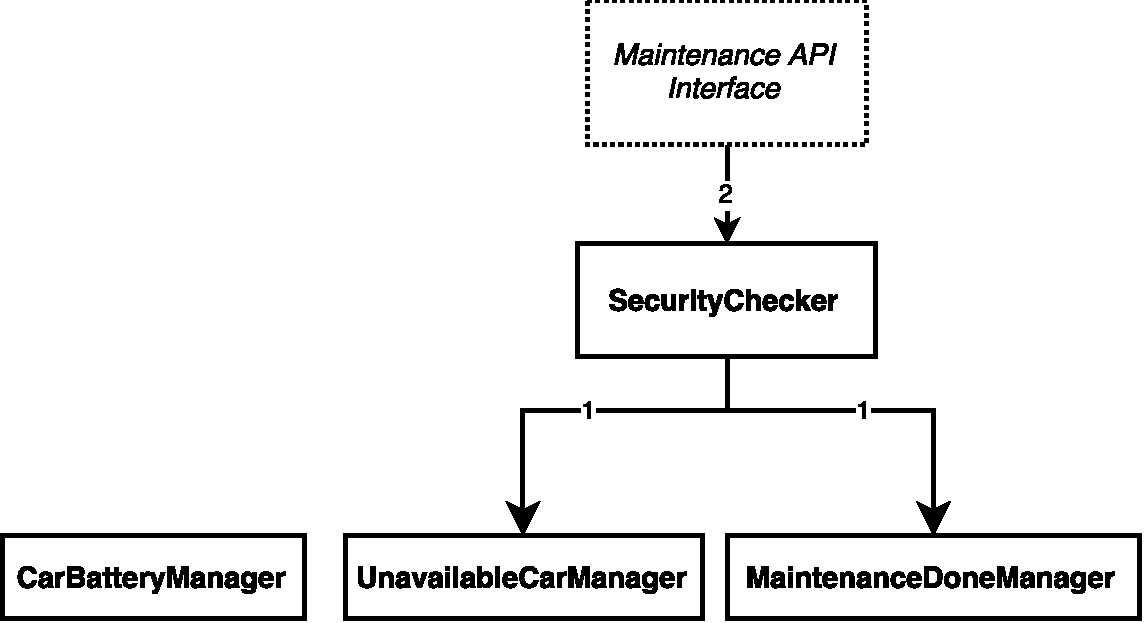
\includegraphics[width=\linewidth]{img/maintenanceIntegration}
			\caption{
				\label{fig:maintenanceIntegration} 
				\emph{MaintenanceManager integration}
			}
		\end{figure}
		
\paragraph{UserInformationManager} 
The diagram above shows the needed precedences in the integration phase inside the \emph{UserInformationManager} component.
\paragraph{}

		\begin{figure}[h]
			\centering
			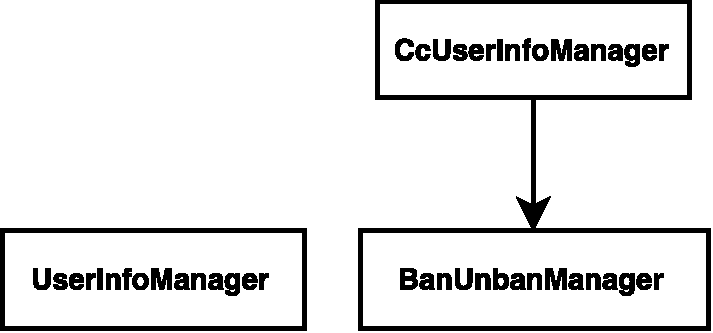
\includegraphics[width=0.6\linewidth]{img/userIntegration}
			\caption{
				\label{fig:userIntegration} 
				\emph{UserInformationManager integration}
			}
		\end{figure}

\subsubsection{Subsystem Integration Sequence}
Identify the order in which subsystems will be integrated; if you have a single subsystem, 2.4.1 and 2.4.2 are to be merged in a single section.
